\documentclass[handout]{beamer}
\let\Tiny=\tiny
\usepackage{hyperref}
\usepackage{amsmath}

% notes
% \setbeameroption{show notes}
% \mode<handout>{
% \usepackage{pgfpages}
% \pgfpagesuselayout{4 on 1}[a4paper, border shrink=5mm, landscape]
% }

\usetheme{default}
\useinnertheme{circles}
\setbeamertemplate{footline}[page number]{}
\setbeamertemplate{navigation symbols}{}
\setbeamertemplate{section in toc}{$\bullet$\hskip1em\inserttocsection\par}
\setbeamertemplate{subsection in toc}{\hskip1.5em$\bullet$\hskip1em\inserttocsubsection\par}
\setbeamertemplate{subsubsection in toc}{\hskip3.75em$\bullet$\hskip1em\inserttocsubsubsection\par}
\setbeamertemplate{enumerate items}[default]

\setbeamercolor{title}{fg=black, bg=gray!30!white}
\setbeamercolor{frametitle}{fg=black, bg=gray!30!white}
\setbeamercolor{normal text}{fg=black}
\setbeamercolor{block title}{fg=black,bg=gray!25!white}
\setbeamercolor{block body}{fg=black,bg=gray!25!white}
\setbeamercolor{alerted text}{fg=gray, bg=black}
\setbeamercolor{itemize item}{fg=gray}
\setbeamercolor{itemize subitem}{fg=gray}
\setbeamercolor{itemize subsubitem}{fg=gray}
\setbeamercolor{enumerate item}{fg=black}
\setbeamercolor{enumerate subitem}{fg=black}
\setbeamercolor{enumerate subsubitem}{fg=black}
\setbeamercolor{section in toc}{bg=gray,fg=black}
\setbeamercolor{section number projected}{fg=black,bg=gray!30!white}

% bib fixes
\setbeamertemplate{bibliography entry title}{}
\setbeamertemplate{bibliography entry location}{}
\setbeamertemplate{bibliography entry note}{}

\newcommand{\vitem}{\vfill\item} 
\newcommand{\fitgraphics}{\includegraphics[width=0.85\textwidth, height=\textheight, keepaspectratio]}
\newtheorem{prop}{Proposition}

% maybe remove
% \AtBeginSection[]
% {
%     \begin{frame}
%     \frametitle{Outline}
%     {\tableofcontents[currentsection]}
%     \end{frame}
% }

\title{3-D Depth Reconstruction from a Single Still Image}
\subtitle{International Journal of Computer Vision (IJCV), Aug 2007}
\author{Ashutosh Saxena, Sung H. Chung, Andrew Y. Ng.}
\date{April 17, 2013}

\begin{document}

% Creates title page of slide show using above information
\begin{frame}
    \titlepage
    \center\noindent Presenter: Yiying Li
\end{frame}

\section[Outline]{}

\begin{frame}
    \frametitle{Outline}
    \tableofcontents
\end{frame}

\section{Motivation}

\begin{frame}[t]\frametitle{Motivation}
    \begin{itemize}
        \item Recovering depth is an important application in scene understanding, robotics, and 3-d reconstruction.
        \vitem<+-> Previous work have been extracting depth using stereopsis, or structure from motion.
        \vitem<+-> Humans use certain monocular cues to indicate depth:
        \begin{itemize}
            \item Texture variation
            \item Gradients
            \item Defocus
            \item Color and haze
        \end{itemize}
    \end{itemize}
\end{frame}

\section{Previous Attempts}
\begin{frame}[t]\frametitle{Previous Attempts}
    \begin{itemize}
        \item Reconstruction for known fixed objects (faces, hands), (Nagai et al. 2002)
        \vitem<+-> Using uniform color and Lambertian surfaces (Many many papers).
        \vitem<+-> Fourier spectrum to compute mean depth (Torralba and Oliva 2002).
        \vitem<+-> Supervised learning for 1-D distance for specific obstacles (Michels et al. 2005).
        \vitem<+-> Fixed sky, ground, vertical regions on the image (Hoeim et al. 2005). No real depth map.
    \end{itemize}
\end{frame}

\section{Methods and Evaluation}
\subsection{Feature Extraction}

\begin{frame}[t]\frametitle{Feature Extraction}
    \begin{itemize}
        \item Monocular cues include: texture variations/gradients, light, haze, defocus, occulsion, know object sizes, and many others.
        \vitem<+-> If we only look at these features at a local scale we miss out on global properties of the image.
        \vitem<+-> Convert to YCbCr color space for separation of intensity and color.
    \end{itemize}
\end{frame}

\begin{frame}[t]\frametitle{Feature Extraction}
    \begin{itemize}
        \item<+-> Absolute Features:
        \begin{itemize}
            \item<+-> Texture information is in the intensity channel.
            \vitem<+-> Law's mask and six rotated edge filters are convolved with intensity.
            \vitem<+-> Haze is usually in low frequency of color channels.
            \vitem<+-> Color channels are convolved with a local averaging filter.
            \vitem<+-> 17 features: 9 Law's, 6 edge, 2 color.
            \vitem<+-> The author also chose to square each filter output as well leaving us with 34 dimensions.
        \end{itemize}
        \item<+-> Relative Features:
        \begin{itemize}
            \vitem 10-bin histogram of each of the 17 filter outputs.
            \vitem 170 dimensions.
        \end{itemize}
    \end{itemize}
\end{frame}

\begin{frame}[t]\frametitle{Features}
    
\includegraphics[width=\linewidth]{lawsmask.PNG}
    \vfill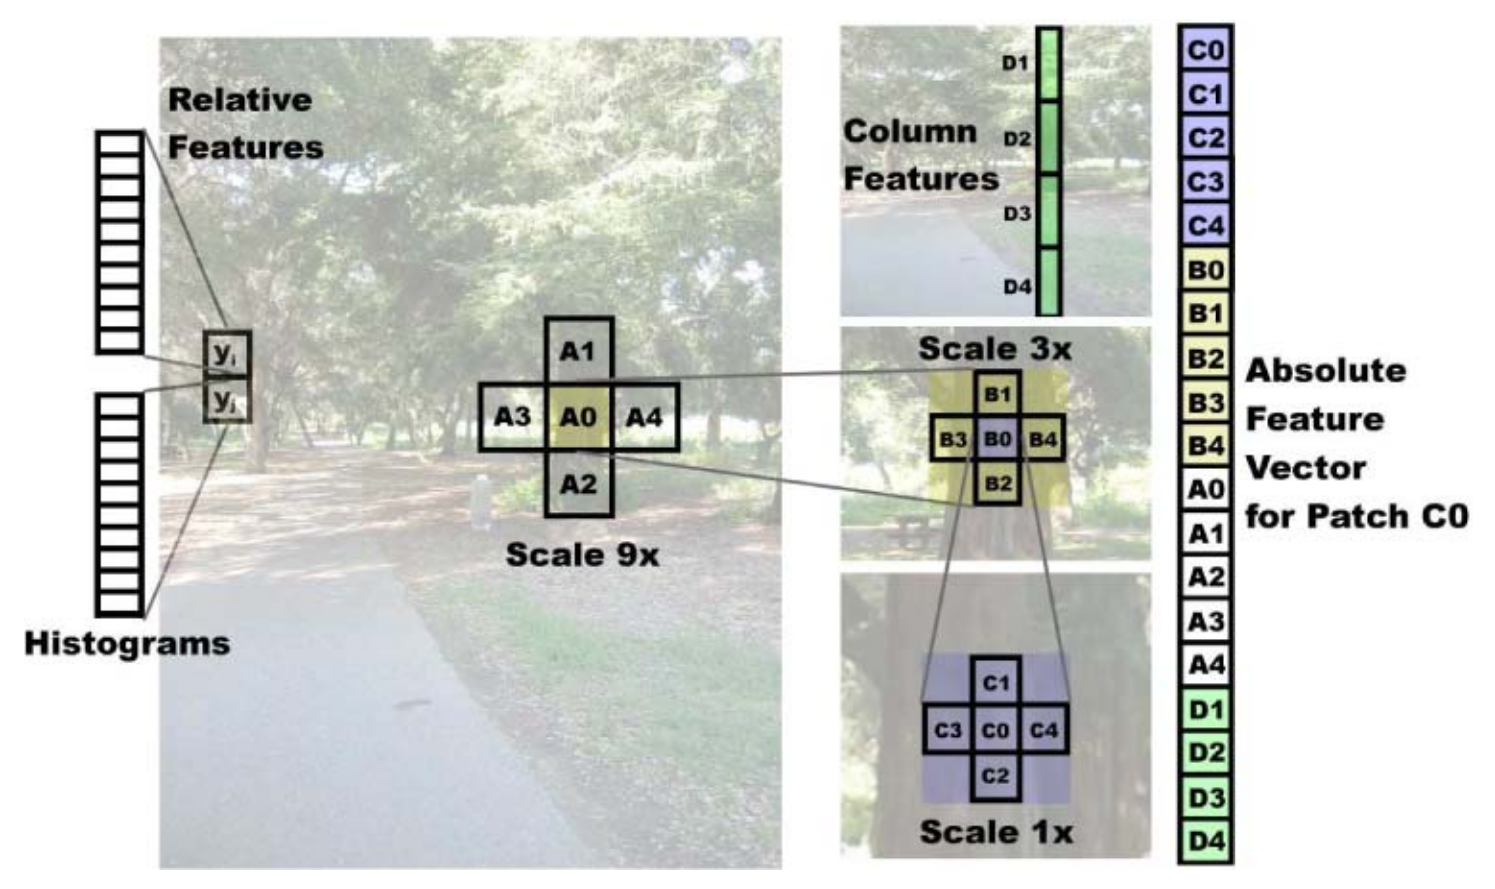
\includegraphics[width=\linewidth]{Features.PNG}
\end{frame}

\begin{frame}[t]\frametitle{Learning Model}
    \begin{itemize}
        \vitem Represented using a multi-scale hierarchal Markov Random Field (MRF).
        \vitem Two different models that only different in inference.
        \vitem Gaussian Model:
    \end{itemize}
    \begin{equation}
    \small
    \begin{split}
    \nonumber
    P_G(d|X; \theta, \sigma) = \frac{1}{Z_G}\exp\left(-\sum_{i=1}^{M}\frac{(d_i(1)-x_i^T\theta_r)^2}{2\sigma^2_{1r}} - \right.\\
    \left.\sum_{s=1}^3\sum_{i=1}^M\sum_{j \in N_s(i)} \frac{(d_i(s)-d_j(s))^2}{2\sigma_{2rs}^2}\right)
    \end{split}
    \end{equation}
    \begin{itemize}
        \vitem Laplacian Model:
    \end{itemize}
    \begin{equation}
    \small
    \begin{split}
    \nonumber
    P_L(d|X; \theta, \lambda) = \frac{1}{Z_L}\exp\left(-\sum_{i=1}^{M}\frac{(d_i(1)-x_i^T\theta_r)^2}{\lambda_{1r}} - \right.\\
    \left.\sum_{s=1}^3\sum_{i=1}^M\sum_{j \in N_s(i)} \frac{|d_i(s)-d_j(s)|}{\lambda_{2rs}}\right)
    \end{split}
    \end{equation}
\end{frame}

\section{Evaluation}
\begin{frame}[t]\frametitle{Evaluation}
    \begin{itemize}
        \vitem Ground truth depth maps are captured by a 3-D laser scanner.
        \vitem Depth maps's are synced to the same FoV of the camera.
        \vitem Various different environments, trees, buildings, etc\dots
        \vitem 400 training pairs.
        \vitem 134 testing pairs.
    \end{itemize}
\end{frame}

\section{Replication}
\begin{frame}[t]\frametitle{Replication Results}
    \begin{itemize}
        \item Replicated using a 8x8 pixel patch in the first scale.
        \vitem Author's mean log 10 error for Gaussian Model: 0.133
        \vitem Replicated mean log 10 error for Gaussian Model: 0.150
        \vitem Replicate mean error: 1.4155 meters
    \end{itemize}
\end{frame}

\begin{frame}[t]\frametitle{Compare Replication Results}
    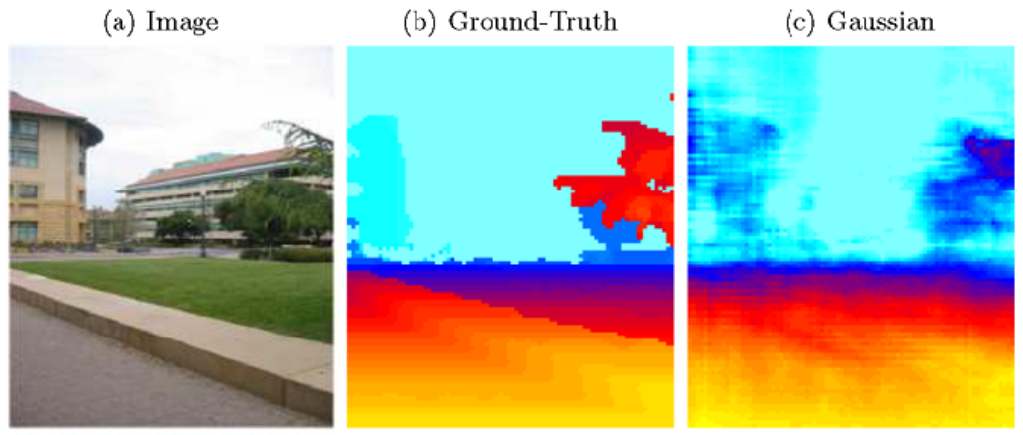
\includegraphics[width=\linewidth]{compare1.png} \\
    \vfill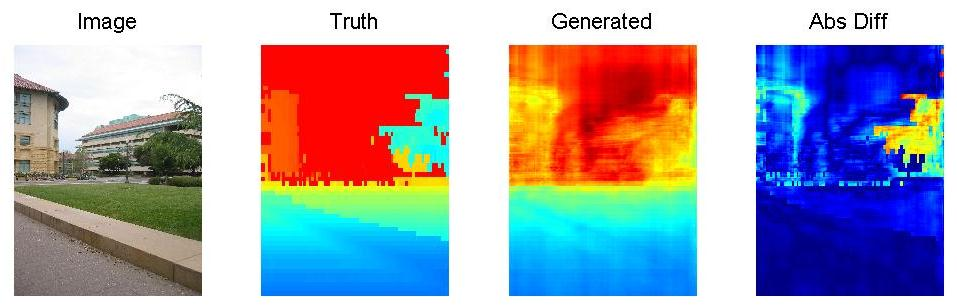
\includegraphics[width=\linewidth]{compare1.jpg}
\end{frame}

\begin{frame}[t]\frametitle{Compare Replication Results}
    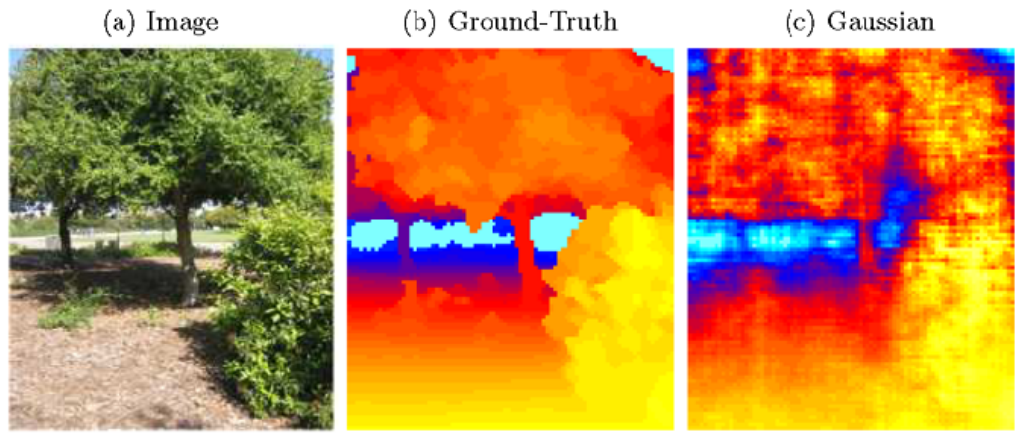
\includegraphics[width=\linewidth]{compare2.png} \\
    \vfill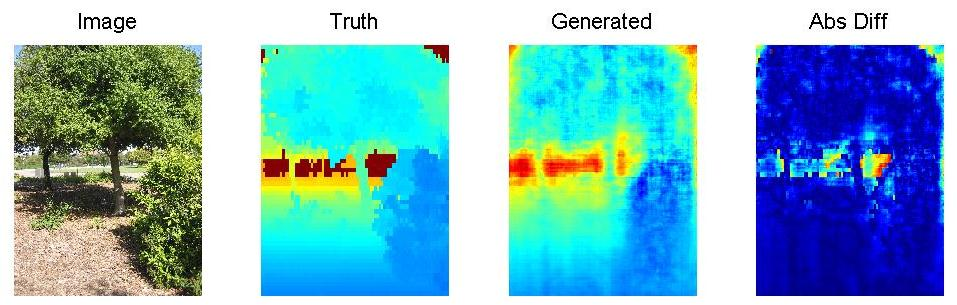
\includegraphics[width=\linewidth]{compare2.jpg}
\end{frame}

\begin{frame}[t]\frametitle{Good Results}
    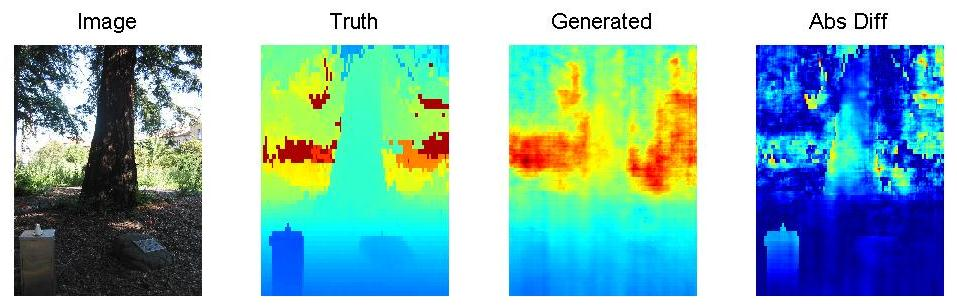
\includegraphics[width=\linewidth]{good1.jpg} \\
    \vfill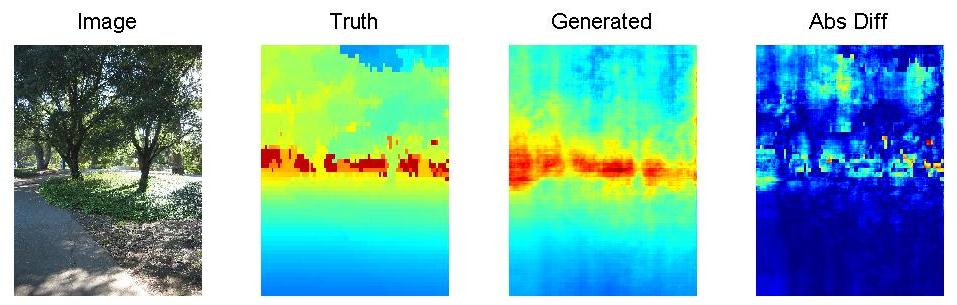
\includegraphics[width=\linewidth]{good2.jpg}
\end{frame}

\begin{frame}[t]\frametitle{Good Results}
    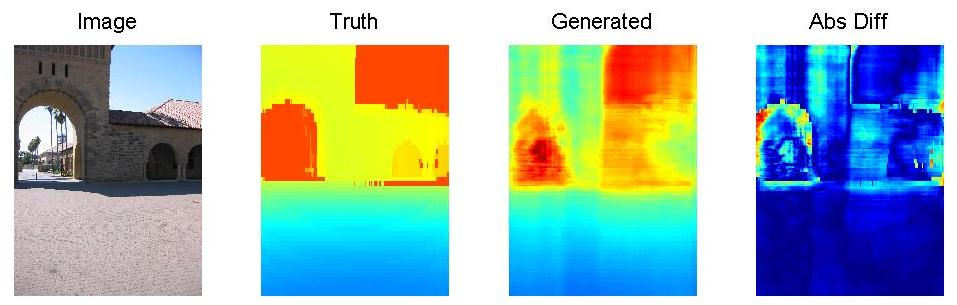
\includegraphics[width=\linewidth]{good3.jpg} \\
    \vfill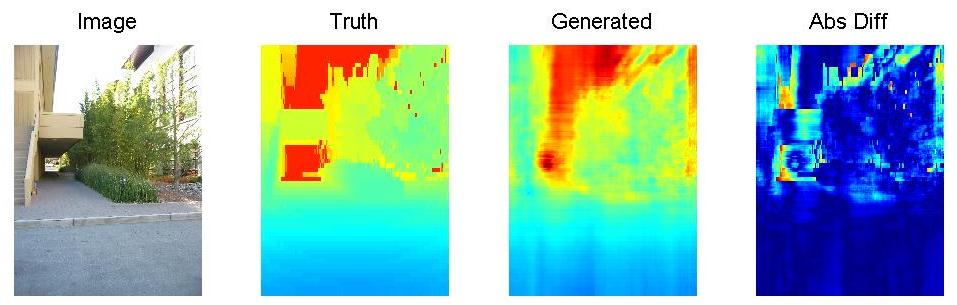
\includegraphics[width=\linewidth]{good4.jpg}
\end{frame}

\begin{frame}[t]\frametitle{Bad Results}
    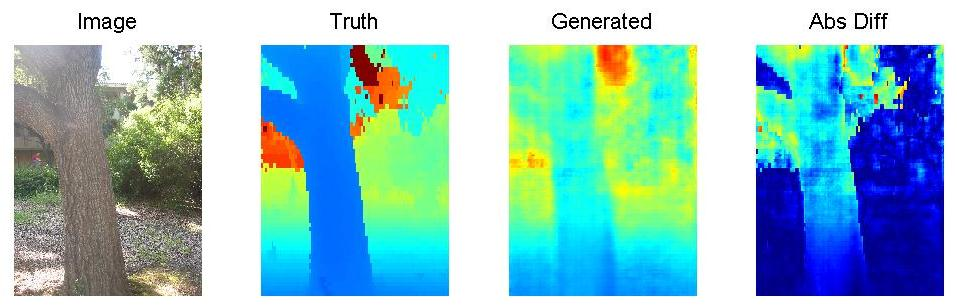
\includegraphics[width=\linewidth]{bad1.jpg} \\
    \vfill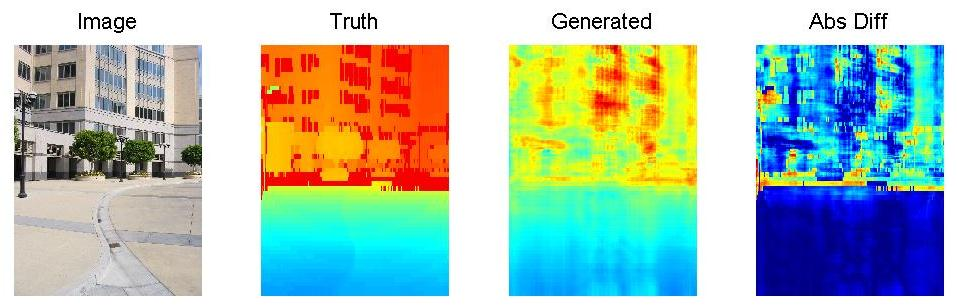
\includegraphics[width=\linewidth]{bad2.jpg}
\end{frame}

\begin{frame}[t]\frametitle{Bad Results}
    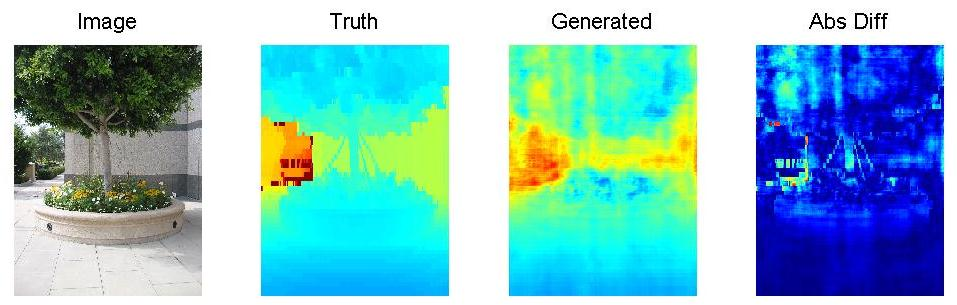
\includegraphics[width=\linewidth]{bad3.jpg} \\
    \vfill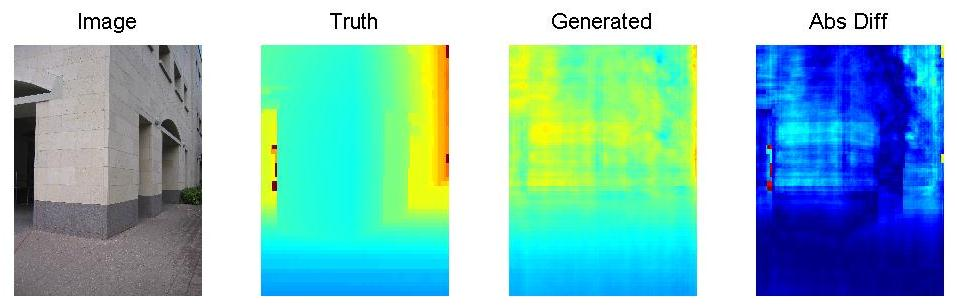
\includegraphics[width=\linewidth]{bad4.jpg}
\end{frame}

\section{Difficulties}
\begin{frame}[t]\frametitle{Difficulties}
    \begin{itemize}
        \item Insurmountable difficulties:
        \begin{itemize}
            \vitem 2nd term dropped from the model as the paper doesn't provide the MAP inference method.
            \vitem Laplacian wasn't successfully implemented, as I couldn't find a correct way to solve the linear program in the MAP inference.
        \end{itemize}
        \item Surmountable difficulties:
        \begin{itemize}
            \vitem The cost to calculate the absolute features of images
            \vitem 1704x2272 image had a feature ``matrix'' that cost about 280MB and without vectorization 300s to compute.
            \vitem With some clever optimizations of pre-computing the require information, this was dropped to 30.
            \vitem Can't load all image features to memory (100+ GB) for training.
            \vitem Loading whole image features costs around 300s and around 400s for linear regression.
            \vitem Save each image's features by rows reduces training time from (3 days to 1.3 days).
        \end{itemize}
    \end{itemize}
\end{frame}

\section{Importance}
\begin{frame}[t]\frametitle{Importance and Future Gold}
    \begin{itemize}
        \item The problem of generating depth is still an extremely interesting problem that humans seems to be much better at.
        \vitem The author takes a interesting approach to generated the right features that has the most information that has a regard to depth. 
        \vitem The value of the author is more as a augmenting method inorder to generate accurate depth maps.
        \vitem The work produces a very general depth map that is extremely useful for simple inferences about the environment.
        \vitem It is interesting to see what other features detctors we can add to possible make this method more robust.
        \vitem It is an good example just how much information a standard image can hold.
        \vitem The method is potentially fast enough given GPU acceleration for real time robotics applications, to augment stereo depth estimation.
    \end{itemize}
\end{frame}
\end{document}